%% LyX 2.2.2 created this file.  For more info, see http://www.lyx.org/.
%% Do not edit unless you really know what you are doing.
\documentclass[ruled]{article}
\usepackage{courier}
\usepackage[latin9]{inputenc}
\usepackage[letterpaper]{geometry}
\geometry{verbose}
\usepackage{color}
\usepackage{algorithm2e}
\usepackage{amsmath}
\usepackage{graphicx}
\usepackage[unicode=true,
 bookmarks=false,
 breaklinks=false,pdfborder={0 0 1},backref=section,colorlinks=true]
 {hyperref}



\makeatletter

%%%%%%%%%%%%%%%%%%%%%%%%%%%%%% LyX specific LaTeX commands.
\providecommand{\LyX}{\texorpdfstring%
  {L\kern-.1667em\lower.25em\hbox{Y}\kern-.125emX\@}
  {LyX}}
%% A simple dot to overcome graphicx limitations
\newcommand{\lyxdot}{.}


\@ifundefined{date}{}{\date{}}
%%%%%%%%%%%%%%%%%%%%%%%%%%%%%% User specified LaTeX commands.
\title{Machine Learning and Computational Statistics, Spring 2017\\
Homework 2: Lasso Regression} 

%\date{Due: February $11^{th}$, 11am}




\usepackage{amsfonts}\usepackage{capt-of}
%\usepackage{url}
\usepackage{color}
\usepackage{bbm}
\usepackage{enumerate}
\newcommand{\carlos}[1]{\textcolor{red}{Carlos: #1}}
\newcommand{\field}[1]{\mathbb{#1}} 
\newcommand{\hide}[1]{#1}
\newcommand{\pd}[2]{\frac{\partial #1}{\partial #2}}
\providecommand{\m}[1]{\mathbf{#1}}
\providecommand{\norm}[1]{\left\|#1\right\|}
\providecommand{\sign}[1]{\text{sign}\left(#1\right)}
\DeclareMathOperator*{\argmin}{arg\,min}
\providecommand{\what}{\m{\hat{w}}}
\providecommand{\dw}{\Delta w}
\providecommand{\dmw}{\Delta \m{w}}
\providecommand{\hy}{\hat{y}}

\usepackage{listings}
\usepackage{color}

\definecolor{dkgreen}{rgb}{0,0.6,0}
\definecolor{gray}{rgb}{0.5,0.5,0.5}
\definecolor{mauve}{rgb}{0.58,0,0.82}

\lstset{frame=tb,
  language=Java,
  aboveskip=3mm,
  belowskip=3mm,
  showstringspaces=false,
  columns=flexible,
  basicstyle={\small\ttfamily},
  numbers=none,
  numberstyle=\tiny\color{gray},
  keywordstyle=\color{blue},
  commentstyle=\color{dkgreen},
  stringstyle=\color{mauve},
  breaklines=true,
  breakatwhitespace=true,
  tabsize=3
}
\makeatother

\begin{document}
\global\long\def\reals{\mathbf{R}}
 \global\long\def\integers{\mathbf{Z}}
 \global\long\def\naturals{\mathbf{N}}
 \global\long\def\rationals{\mathbf{Q}}
 \global\long\def\ca{\mathcal{A}}
 \global\long\def\cb{\mathcal{B}}
 \global\long\def\cc{\mathcal{C}}
 \global\long\def\cd{\mathcal{D}}
 \global\long\def\ce{\mathcal{E}}
 \global\long\def\cf{\mathcal{F}}
 \global\long\def\cg{\mathcal{G}}
 \global\long\def\ch{\mathcal{H}}
 \global\long\def\ci{\mathcal{I}}
 \global\long\def\cj{\mathcal{J}}
 \global\long\def\ck{\mathcal{K}}
 \global\long\def\cl{\mathcal{L}}
 \global\long\def\cm{\mathcal{M}}
 \global\long\def\cn{\mathcal{N}}
 \global\long\def\co{\mathcal{O}}
 \global\long\def\cp{\mathcal{P}}
 \global\long\def\cq{\mathcal{Q}}
 \global\long\def\calr{\mathcal{R}}
 \global\long\def\cs{\mathcal{S}}
 \global\long\def\ct{\mathcal{T}}
 \global\long\def\cu{\mathcal{U}}
 \global\long\def\cv{\mathcal{V}}
 \global\long\def\cw{\mathcal{W}}
 \global\long\def\cx{\mathcal{X}}
 \global\long\def\cy{\mathcal{Y}}
 \global\long\def\cz{\mathcal{Z}}
 \global\long\def\ind#1{1(#1)}
 \global\long\def\pr{\mathbb{P}}
 \global\long\def\predsp{\cy}
 \global\long\def\outsp{\cy}
 \global\long\def\prxy{P_{\cx\times\cy}}
 \global\long\def\prx{P_{\cx}}
 \global\long\def\prygivenx{P_{\cy\mid\cx}}
 \global\long\def\ex{\mathbb{E}}
 \global\long\def\var{\textrm{Var}}
 \global\long\def\cov{\textrm{Cov}}
 \global\long\def\sgn{\textrm{sgn}}
 \global\long\def\sign{\textrm{sign}}
 \global\long\def\kl{\textrm{KL}}
 \global\long\def\law{\mathcal{L}}
 \global\long\def\eps{\varepsilon}
 \global\long\def\as{\textrm{ a.s.}}
 \global\long\def\io{\textrm{ i.o.}}
 \global\long\def\ev{\textrm{ ev.}}
 \global\long\def\convd{\stackrel{d}{\to}}
 \global\long\def\eqd{\stackrel{d}{=}}
 \global\long\def\del{\nabla}
 \global\long\def\loss{\ell}
 \global\long\def\risk{R}
 \global\long\def\emprisk{\hat{R}_{\ell}}
 \global\long\def\lossfnl{L}
 \global\long\def\emplossfnl{\hat{L}}
 \global\long\def\empminimizer#1{\hat{#1}_{\ell}}
 \global\long\def\minimizer#1{#1_{*}}
 \global\long\def\etal{\textrm{et. al.}}
 \global\long\def\tr{\operatorname{tr}}
 \global\long\def\trace{\operatorname{trace}}
 \global\long\def\diag{\text{diag}}
 \global\long\def\rank{\text{rank}}
 \global\long\def\linspan{\text{span}}
 \global\long\def\proj{\text{Proj}}
 \global\long\def\argmax{\operatornamewithlimits{arg\, max}}
 \global\long\def\argmin{\operatornamewithlimits{arg\, min}}
 \global\long\def\bfx{\mathbf{x}}
 \global\long\def\bfy{\mathbf{y}}
 \global\long\def\bfl{\mathbf{\lambda}}
 \global\long\def\bfm{\mathbf{\mu}}
 \global\long\def\calL{\mathcal{L}}
 \global\long\def\vw{\boldsymbol{w}}
 \global\long\def\vx{\boldsymbol{x}}
 \global\long\def\vxi{\boldsymbol{\xi}}
 \global\long\def\valpha{\boldsymbol{\alpha}}
 \global\long\def\vbeta{\boldsymbol{\beta}}
 \global\long\def\vsigma{\boldsymbol{\sigma}}
 \global\long\def\vmu{\boldsymbol{\mu}}
 \global\long\def\vtheta{\boldsymbol{\theta}}
 \global\long\def\vd{\boldsymbol{d}}
 \global\long\def\vs{\boldsymbol{s}}
 \global\long\def\vt{\boldsymbol{t}}
 \global\long\def\vh{\boldsymbol{h}}
 \global\long\def\ve{\boldsymbol{e}}
 \global\long\def\vf{\boldsymbol{f}}
 \global\long\def\vg{\boldsymbol{g}}
 \global\long\def\vz{\boldsymbol{z}}
 \global\long\def\vk{\boldsymbol{k}}
 \global\long\def\va{\boldsymbol{a}}
 \global\long\def\vb{\boldsymbol{b}}
 \global\long\def\vv{\boldsymbol{v}}
 \global\long\def\vy{\boldsymbol{y}}
 \global\long\def\hil{\ch}
 \global\long\def\rkhs{\hil}
 \maketitle

\textbf{Saturday, February 11, 2017}
\textbf{Yidi Zhang}


\section{Introduce}
\section{Ridge Regression}%2

By construction, we know that our dataset admits a sparse solution.
Here, we want to evaluate the performance of ridge regression (i.e.
$\ell_{2}$-regularized linear regression) on this dataset.
\begin{enumerate}
\item Run ridge regression on this dataset. Choose the $\lambda$ that minimizes
the square loss on the validation set. For the chosen $\lambda$,
examine the model coefficients. Report on how many components with
true value $0$ have been estimated to be non-zero, and vice-versa
(don't worry if they are all nonzero). Now choose a small threshold
(say $10^{-3}$ or smaller), count anything with magnitude smaller
than the threshold as zero, and repeat the report. (For running ridge
regression, you may either use your code from HW1, or you may use
\texttt{scipy.optimize.minimize} (see the demo code provided for guidance).
For debugging purposes, you are welcome, even encouraged, to compare
your results to what you get from \texttt{sklearn.linear\_model.Ridge}.) 
\end{enumerate}
{\bfseries Answer 2.1:}%2.1

\begin{lstlisting}
import numpy as np
from scipy.optimize import minimize

X = np.loadtxt("/Users/twff/Downloads/machine learning/hw/hw2-lasso/data/X_train.txt")
y = np.loadtxt("/Users/twff/Downloads/machine learning/hw/hw2-lasso/data/y_train.txt")
X_valid = np.loadtxt("/Users/twff/Downloads/machine learning/hw/hw2-lasso/data/X_valid.txt")
y_valid = np.loadtxt("/Users/twff/Downloads/machine learning/hw/hw2-lasso/data/y_valid.txt")

(N,D) = X_train.shape

w = np.random.rand(D,1)

def ridge(Lambda):
    def ridge_obj(theta):
        return ((np.linalg.norm(np.dot(X, theta) - y))**2)/(2*N) + Lambda*(np.linalg.norm(theta))**2
    return ridge_obj

def compute_loss(X, y, Lambda, theta):
    (N,D) = X.shape
    return ((np.linalg.norm(np.dot(X, theta) - y))**2)/(2*N)

for i in range(-8,6):
    Lambda = 10**i;
    w_opt = minimize(ridge(Lambda), w)
    print(Lambda, compute_loss(X_valid, y_valid, Lambda, w_opt.x))
\end{lstlisting}

When $\lambda = 1e-09 $, it can minimize the square loss, which is 0.0587394466821.
$\lambda = 1e-09 $, 0 component with true value 0 has been estimated to be non-zero. And when choosing a small threshold which equals to $10^{-3}$, the number is 50.

\begin{lstlisting}
w_opt = minimize(ridge(1e-5), w)
len(w_opt.x[w_opt.x==0])
len(w_opt.x[w_opt.x <= 0.001])
\end{lstlisting}

When comparing the results with the one using \texttt{sklearn.linear\_model.Ridge}, the square loss is similar, which is 0.10057515598174918 when $\lambda = 1e-5$, so the code do not have bug.
\begin{lstlisting}
from sklearn.linear_model import Ridge
clf = Ridge(alpha=1e-5)
clf.fit(X, y)
a = clf.predict(X)#numpy.dot(X,theta)
a =((np.linalg.norm(a - y))**2)/(2*N)
b = compute_loss(X_valid, y_valid, Lambda, w_opt.x)
b
\end{lstlisting}
{}

\pagebreak
\section{\label{subsec:Shooting-algorithm}Coordinate Descent for Lasso (a.k.a.
The Shooting algorithm)}%3

\subsection{Experiments with the Shooting Algorithm}%3.1
\begin{enumerate}
\item Write a function that computes the Lasso solution for a given $\lambda$
using the shooting algorithm described above. This function should
take a starting point for the optimization as a parameter. Run it
on the dataset constructed in (1.1), and select the $\lambda$ that
minimizes the square error on the validation set. Report the optimal
value of $\lambda$ found, and the corresponding test error. Plot
the validation error vs $\lambda$. {[}Don't use the homotopy method
in this part, as we want to measure the speed improvement of homotopy
methods in question \ref{enu:homotopy}. Also, no need to vectorize
the calculations until question \ref{enu:vectorization}, where again
we'll compare the speedup. In any case, having two different implementations
of the same thing is a good way to check your work.{]}%%%%%3.1.1

{\bfseries Answer 3.1.1:}
\begin{lstlisting}
def lassoShooting(X, y, lambda_reg, w, ep = 1e-6, iter_max=1000):
    (n,p) = X.shape
    converge = True
    itera = 0
    
    while converge and (itera + 1) <= iter_max:
        w_old = w.copy()
        for j in range(p):
            a = []
            c = []
            for i in range(n):
                aj = 2 * X[i,j]*X[i,j]
                cj = 2 * X[i,j]*(y[i]-np.dot(w.T,X[i]) + X[i,j]*w[j])
                a.append(aj)
                c.append(cj)
            aj_sum = sum(a)
            cj_sum = sum(c)
            w[j] = soft(cj_sum/aj_sum, lambda_reg/aj_sum)
        converge = (sum(abs(w-w_old)) >= ep)
        #print(sum(abs(w-w_old)))
        itera +=1
    print(itera)
    return w

def soft(a, b):
    if a <- b:
        c = a+b
    elif a > b:
        c = a - b
    else:
        c = 0
    return c
    \end{lstlisting}

\begin{lstlisting}
import matplotlib.pyplot as plt
%matplotlib inline

w = np.zeros(X.shape[1])
loss = []
for i in range(-5,2):
    Lambda = 10**i;
    w_opt = lassoShooting(X, y, lambda_reg=Lambda, w=w, ep=1e-3)
    loss.append(compute_loss(X_valid, y_valid, Lambda, w_opt))
    print(Lambda, compute_loss(X_valid, y_valid, Lambda, w_opt))

plt.plot(range(-5,2), loss)
plt.xlabel("lambda")
plt.ylabel("Loss")
plt.savefig("/Users/twff/Downloads/machine learning/hw/hw2-lasso/img311")
\end{lstlisting}

\begin{figure}
  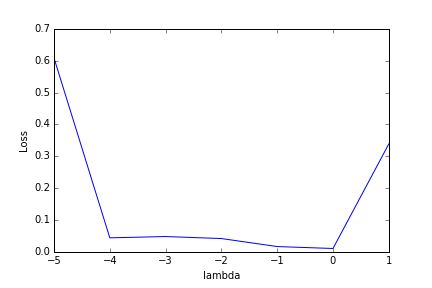
\includegraphics[width=\linewidth]{img311.png}
  \caption{Objective function for each step size.}
  \label{fig:311}
\end{figure}

\begin{lstlisting}
w = np.zeros(X.shape[1])
w_opt = lassoShooting(X, y, lambda_reg=0.4, w=w, ep=1e-3)
compute_loss(X_test, y_test, 0.4 ,w_opt)
\end{lstlisting}

And I found the minimum square loss is between 0 and 1. After zooming in, the optimal $\lambda$ found is 0.4, and the corresponding test error is 0.0093066225296064235.

\begin{lstlisting}
w = np.zeros(X.shape[1])
lambda_reg = np.linspace(0,1,10)
loss = []
for i in range(len(lambda_reg)):
    w_opt = lassoShooting(X, y, lambda_reg=lambda_reg[i], w=w, ep=1e-3)
    loss.append(compute_loss(X_valid, y_valid, lambda_reg[i], w_opt))
    print(lambda_reg[i], compute_loss(X_valid, y_valid, lambda_reg[i], w_opt))

plt.plot(lambda_reg, loss)
plt.xlabel("lambda")
plt.ylabel("Loss")
plt.savefig("/Users/twff/Downloads/machine learning/hw/hw2-lasso/img311b")
\end{lstlisting}

\begin{figure}
  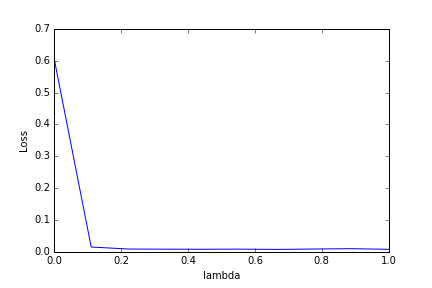
\includegraphics[width=\linewidth]{img311b.png}
  \caption{Objective function for each step size.}
  \label{fig:311b}
\end{figure}

\pagebreak
\item Analyze the sparsity\footnote{One might hope that the solution will a sparsity pattern that is similar
to the ground truth. Estimators that preserve the sparsity pattern
(with enough training data) are said to be \textbf{``sparsistent''}
(sparse + consistent). Formally, an estimator $\hat{\beta}$ of parameter
$\beta$ is said to be consistent if the estimator $\hat{\beta}$
converges to the true value $\beta$ in probability as our sample
size goes to infinity. Analogously, if we define the support of a
vector $\beta$ as the indices with non-zero components, i.e. $\text{Supp}(\beta)=\{j\mid\beta_{j}\neq0\}$,
then an estimator $\hat{\beta}$ is said to be sparsistent if as the
number of samples becomes large, the support of $\hat{\beta}$ converges
to the support of $\beta$, or ${\displaystyle \lim_{m\rightarrow\infty}P[\text{Supp}(\hat{\beta}_{m})=\text{Supp}(\beta)]}$
= 1. } of your solution, reporting how many components with true value zero
have been estimated to be non-zero, and vice-versa.%%%%%%3.1.2

{\bfseries Answer 3.1.2:}
\begin{lstlisting}
w = np.zeros(X.shape[1])
w_opt = lassoShooting(X, y, lambda_reg=0.4, w=w, ep=1e-3)
compute_loss(X_test, y_test, 0.4 ,w_opt)
\end{lstlisting}
0 components with true value zero has been estimated to be non-zero. But if the threshold is $10^{-3}$, the number would be 51. In this case, we can see the solution above as a sparsity pattern. 

\pagebreak 
\item \label{enu:homotopy}Implement the homotopy method described above.
Compare the runtime for computing the full regularization path (for
the same set of $\lambda$'s you tried in the first question above)
using the homotopy method compared to the basic shooting algorithm.%%%%%%3.1.3

{\bfseries Answer 3.1.3:}
\begin{lstlisting}
def lassoShooting_homotopy(X, y, w, ep = 1e-3, pa=0.1,iter_max=2000):
    lambda_max = 2 * np.linalg.norm(np.dot(X.T, y), np.inf)
    (n,p) = X.shape
    converge = True
    itera = 0
    lambda_reg = 1000
    lambda_old = 0
    lambda_list = []
    loss = []
    w = np.zeros(p)
    #print(w)
    
    while np.abs(lambda_old - lambda_reg)>ep:
        w_prev = w.copy()
        w_new = lassoShooting(X, y, lambda_reg, w, ep = 1e-3, iter_max=iter_max)
        #print(w_new)
        loss.append(compute_loss(X_valid, y_valid, lambda_reg, w_new))
        lambda_list.append(lambda_reg)
        if(sum(abs(w_prev-w_new)) < ep):
            #print(sum(abs(w-w_new)))
            break
        w = w_new.copy()
        lambda_reg = pa*lambda_reg
        
    return lambda_list, loss
\end{lstlisting}
The homotopy method time is 124.1882728970013? while the regular method time is 302.8984123150003.



\pagebreak
\item \label{enu:vectorization}The algorithm as described above is not
ready for a large dataset (at least if it has been implemented in
basic Python) because of the implied loop over the dataset (i.e. where
we sum over the training set). By using matrix and vector operations,
we can eliminate the loops. This is called ``vectorization'' and
can lead to dramatic speedup in languages such as Python, Matlab,
and R. Derive matrix expressions for computing $a_{j}$ and $c_{j}$.
(Hint: A matlab version of this vectorized method can be found in
the assignment zip file.) Implement the matrix expressions and measure
the speedup in computing the regularization path. %%%%%3.1.4

{\bfseries Answer 3.1.4:}
\begin{lstlisting}
def lassoShooting_matrix(X, y, lambda_reg, w, ep = 1e-3, iter_max=500):
    (n,p) = X.shape
    w_opt = w
    converge = True
    itera = 0
    
    while converge and (itera+1) <= iter_max:
        w_old = w.copy()
        a = np.dot(X.T, X)
        for j in range(p):
            a = 2*X[:,j].dot(X[:,j])
            c = 2*X[:,j].dot(y) - 2* X.dot(w).dot(X[:,j]) +  2*X[:,j].dot(X[:,j])*w[j]
            w[j] = soft(c/a, lambda_reg/a)
        converge = (sum(abs(w-w_old)) >= ep)
        #print(sum(abs(w-w_old)))
        itera +=1
    return w
    \end{lstlisting}

For $\lambda = 0.4$, the regular lasso shooting method time is 20.220894887999748, but the vectorization method time is 0.46611224899970694. For computing the regularization path, vectorization time is 9.962034545998904, and regular time is 302.8984123150003.

\end{enumerate}


\pagebreak
\subsection{Deriving the Coordinate Minimizer for Lasso}

This problem is to derive the expressions for the coordinate minimizers
used in the Shooting algorithm. This is often \href{http://davidrosenberg.github.io/mlcourse/Archive/2015/Lectures/2.Lab.subgradient-descent.pdf\#page=15}{derived using subgradients (slide 15)},
but here we will take a bare hands approach (which is essentially
equivalent). 

In each step of the shooting algorithm, we would like to find the
$w_{j}$ minimizing
\begin{eqnarray*}
f(w_{j}) & = & \sum_{i=1}^{n}\left(w^{T}x_{i}-y_{i}\right)^{2}+\lambda\left|w\right|_{1}\\
 & = & \sum_{i=1}^{n}\left[w_{j}x_{ij}+\sum_{k\neq j}w_{k}x_{ik}-y_{i}\right]^{2}+\lambda\left|w_{j}\right|+\lambda\sum_{k\neq j}\left|w_{k}\right|,
\end{eqnarray*}
where we've written $x_{ij}$ for the $j$th entry of the vector $x_{i}$.
This function is strictly convex in $w_{j}$, and thus it has a unique
minimum. The only thing keeping $f$ from being differentiable is
the term with $\left|w_{j}\right|$. So $f$ is differentiable everywhere
except $w_{j}=0$. We'll break this problem into 3 cases: $w_{j}>0$,
$w_{j}<0$, and $w_{j}=0$. In the first two cases, we can simply
differentiate $f$ w.r.t. $w_{j}$ to get optimality conditions. For
the last case, we'll use the fact that since $f:\reals\to\reals$
is convex, 0 is a minimizer of $f$ iff
\[
\lim_{\eps\downarrow0}\frac{f(\eps)-f(0)}{\eps}\ge0\quad\mbox{and}\quad\lim_{\eps\downarrow0}\frac{f(-\eps)-f(0)}{\eps}\ge0.
\]
This is a special case of the optimality conditions described in \href{http://davidrosenberg.github.io/mlcourse/Archive/2015/Lectures/5.Lab.misc.pdf\#page=12}{slide 12 here},
where now the ``direction'' $v$ is simply taken to be the scalars
$1$ and $-1$, respectively. 
\begin{enumerate}
\item First let's get a trivial case out of the way. If $x_{ij}=0$ for
$i=1,\ldots,n$, what is the coordinate minimizer $w_{j}$? In the
remaining questions below, you may assume that $\sum_{i=1}^{n}x_{ij}^{2}>0$.%%%%%%3.2.1

{\bfseries Answer 3.2.1:}
If $x_{ij}=0$ for $i=1,\ldots,n$
$$a_{j} = 2\sum_{i=1}^{n}x_{ij}^{2}=0$$, 
$$c_{j} =2\sum_{i=1}^{n}x_{ij}\left(y_{i}-\sum_{k\neq j}w_{k}x_{ik}\right)=0$$ 
thus when $a_{j} = c_{j} = 0$, we can get $w_{j}=0$.

\pagebreak
\item Give an expression for the derivative $f(w_{j})$ for $w_{j}\neq0$.
It will be convenient to write your expression in terms of the following
definitions:
\begin{eqnarray*}
\sign(w_{j}) & := & \begin{cases}
1 & w_{j}>0\\
0 & w_{j}=0\\
-1 & w_{j}<0
\end{cases}\\
a_{j} & := & 2\sum_{i=1}^{n}x_{ij}^{2}\\
c_{j} & := & 2\sum_{i=1}^{n}x_{ij}\left(y_{i}-\sum_{k\neq j}w_{k}x_{ik}\right).
\end{eqnarray*}%%%%3.2.2

{\bfseries Answer 3.2.2:}
$$w_{j} = \sign(w_{j})(|\frac{c_{j}}{a_{j}}|-\frac{\lambda}{a_{j}})$$

for $w_{j}\neq0$:
\begin{eqnarray*}
f(w_{j}) & := & \begin{cases}
\frac{1}{a_{j}} (c_{j}-\lambda)& w_{j}>0\\
\frac{1}{a_{j}} (c_{j}+\lambda) & w_{j}<0
\end{cases}\\
\end{eqnarray*}

\pagebreak
\item If $w_{j}>0$ and minimizes $f$, show that $w_{j}=\frac{1}{a_{j}}\left(c_{j}-\lambda\right)$.
Similarly, if $w_{j}<0$ and minimizes $f$, show that $w_{j}=\frac{1}{a_{j}}\left(c_{j}+\lambda\right)$.
Give conditions on $c_{j}$ that imply that a minimizer $w_{j}$ is
positive and conditions for which a minimizer $w_{j}$ is negative.%%%%%%3.2.3

{\bfseries Answer 3.2.3:}

if $w_{j}>0$, $w_{j} = 1\frac{1}{a_{j}}(|c_{j}|-\lambda)=w_{j} = \frac{1}{a_{j}}(c_{j}-\lambda)$, in this case, $c_{j}$ must bigger than $\lambda$.

if $w_{j}<0$, $w_{j} = -1\frac{1}{a_{j}}(|c_{j}|-\lambda)=w_{j} = \frac{1}{a_{j}}(c_{j}+\lambda)$, in this case, $c_{j}$ must smaller than $-\lambda$.

Give the condition on $c_{j}$ to imply $w_{j}$:

\begin{eqnarray*}
f(w_{j}) & := & \begin{cases}
\frac{1}{a_{j}} (c_{j}-\lambda)>0& if  c_{j}>\lambda\\
\frac{1}{a_{j}} (c_{j}+\lambda)<0 & if  c_{j}<-\lambda\\
w_{j}=0 & otherwise
\end{cases}\\
\end{eqnarray*}

\pagebreak
\item Derive expressions for the two one-sided derivatives at $f(0)$, and
show that $c_{j}\in\left[-\lambda,\lambda\right]$ implies that $w_{j}=0$
is a minimizer.%%%%%%%3.2.4

{\bfseries Answer 3.2.4:}

When $w_{j}>0$, for $c_{j}>\lambda$, suppose $\eps>0$
\[
\lim_{\eps\downarrow0}\frac{f(\eps)-f(0)}{\eps}\ge0.
\]
When $w_{j}<0$, for $c_{j}<-\lambda$
\[
\lim_{\eps\downarrow0}\frac{f(-\eps)-f(0)}{\eps}\ge0.
\]
But if $c_{j}\in\left[-\lambda,\lambda\right]$
\[
\lim_{\eps\downarrow0}\frac{f(\eps)-f(0)}{\eps}\le0\quad\mbox{and}\quad\lim_{\eps\downarrow0}\frac{f(-\eps)-f(0)}{\eps}\le0.
\]
Putting together the preceding expressions, we can conclude that $c_{j}\in\left[-\lambda,\lambda\right]$ implies that $w_{j}=0$ is a minimizer.
\pagebreak
\item Putting together the preceding results, we conclude the following:
\[
w_{j}=\begin{cases}
\frac{1}{a_{j}}\left(c_{j}-\lambda\right) & c_{j}>\lambda\\
0 & c_{j}\in[-\lambda,\lambda]\\
\frac{1}{a_{j}}\left(c_{j}+\lambda\right) & c_{j}<-\lambda
\end{cases}
\]
Show that this is equivalent to the expression given in \ref{subsec:Shooting-algorithm}.\\%%%%3.2.5

{\bfseries Answer 3.2.5:}

\begin{align*}
&\hat{w}={\displaystyle \argmin_{w\in\reals^{d}}\sum_{i=1}^{m}(h_{w}(x_{i})-y_{i})^{2}+\lambda\|w\|_{1}}\\
&f(\hat{w})=\sum_{i=1}^{m}(h_{w}(x_{i})-y_{i})^{2}+\lambda\|w\|_{1}\\
&=g(w)+\lambda\|w\|_{1}
\end{align*}
The derivate of $g(w)$ is:
\begin{align*}
&\del_{w}g(w)=2\sum_{i}^{n}(\sum_{k}^{p}x_{ik}w-y_{i})x_{ij}\\
&=-2\sum_{i}^{n}(y_{i}-\sum_{k}^{p}x_{ik}w)x_{ij}\\
&=-c_{j}
\end{align*}
Then we can get:
\begin{align*}
&g(w_{j+1}) = g(w_{j})+\lambda\del_{w}g(w)+\frac{a_{j}}{2}\\
\end{align*}
The minimizer of $w$ then is given by:
\begin{align*}
&\hat{w} = \sign(w_{j})\left(w_{j}; \frac{\del_{j}g(w)-\lambda}{a_{j}}, \frac{\del_{j}g(w)+\lambda}{a_{j}}\right)\\
& =\sign(w_{j})\left(w_{j}; \frac{c_{j}-\lambda}{a_{j}}, \frac{c_{j}+\lambda}{a_{j}}\right)
\end{align*}
Putting together the preceding results, we can conclude that :
\[
w_{j}=\begin{cases}
\frac{1}{a_{j}}\left(c_{j}-\lambda\right) & c_{j}>\lambda\\
0 & c_{j}\in[-\lambda,\lambda]\\
\frac{1}{a_{j}}\left(c_{j}+\lambda\right) & c_{j}<-\lambda
\end{cases}
\]
is equivalent to the expression:
$$\hat{w}={\displaystyle \argmin_{w\in\reals^{d}}\sum_{i=1}^{m}(h_{w}(x_{i})-y_{i})^{2}+\lambda\|w\|_{1}}$$


\end{enumerate}

\pagebreak
\section{Lasso Properties}%%%%%%4%%%%%%%%%%%%%%%%%%%%%%%

\subsection{Deriving $\lambda_{\mbox{max}}$}%%%%%%%%%%%%4.1

In this problem we will derive an expression for $\lambda_{\text{max}}$.
For the first three parts, use the Lasso objective function excluding
the bias term i.e, $L(w)=\left\Vert Xw-y\right\Vert _{2}^{2}+\lambda\left\Vert w\right\Vert _{1}$.
Show that for any $\lambda\geq2\|X^{T}y\|_{\infty}$, the estimated
weight vector $\hat{w}$ is entirely zero, where $\|\cdot\|_{\infty}$
is the infinity norm (or supremum norm), which is the maximum absolute
value of any component of the vector. 
\begin{enumerate}
\item The one-sided directional derivative of $f(x)$ at $x$ in the direction
$v$ is defined as:
\[
f'(x;v)=\lim_{h\downarrow0}\frac{f(x+hv)-f(x)}{h}
\]
Compute $L'(0;v)$. That is, compute the one-sided directional derivative
of $L(w)$ at $w=0$ in the direction $v$. {[}Hint: the result should
be in terms of $X,y,\lambda,\text{ and }v$.{]}\\
\textbf{}\\%%%%%%%4.1

{\bfseries Answer 4.1.1:}

\begin{align*}
&l'(0;v)=\lim_{h\downarrow0}\frac{l(0+hv)-l(x)}{h},\\
&=  \lim_{h\downarrow0}\frac{(Xhv-y)(Xhv-y)^{T}+\lambda hv-y^{T}y}{h}\\
&=  -2X^{T}v^{T}y+\lambda||v||_{1}
\end{align*}

\pagebreak
\item Since the Lasso objective is convex, for $w^{*}$ to be a minimizer
of $L(w)$ we must have that the directional derivative $L'(w^{*};v)\geq0$
for all $v$. Starting from the condition $L'(0;v)\ge0$, rearrange
terms to get a lower bounds on $\lambda$. {[}Hint: this should be
in terms of $X,y,\text{{and} }v$.{]} \textbf{}\\%%%%%%%%4.1.2

{\bfseries Answer 4.1.2:}

To make $l'(0;v)\geq0$, 
\begin{eqnarray*}
&-2X^{T}v^{T}y+\lambda||v||_{1}\geq0\\
&\lambda||v||_{1}\geq2X^{T}v^{T}y\\
&\lambda\geq\frac{2X^{T}v^{T}y}{||v||_{1}}
\end{eqnarray*}
Thus, the lower bound of $\lambda$ is $\frac{2X^{T}v^{T}y}{||v||_{1}}$

\pagebreak
\item In the previous problem, we get a different lower bound on $\lambda$
for each choice of $v$. Compute the maximum lower bound of $\lambda$
by maximizing the expression over $v.$ Show that this expression
is equivalent to $\lambda_{\text{max}}=2\|X^{T}y\|_{\infty}$.\\%%%%%%%%%4.1.3

{\bfseries Answer 4.1.3:}

\begin{align*}
& \lambda\geq\frac{2X^{T}v^{T}y}{||v||_{1}} \\
& \lambda\geq2\frac{v^{T}}{||v||_{1}} X^{T}y\\
\end{align*}
Suppose $z^{T}=\frac{v^{T}}{||v||_{1}}$, we can get $||z||_{1}=||\frac{v^{T}}{||v||_{1}}||_{1}=\frac{||v||_{1}}{||v||_{1}}=1$.
We let $p=X^{T}y$, then:
\begin{align*}
& z^{T}p=\sum^{n}_{i=1}z_{i}p_{i}\\
& z^{T}p\leq\sum^{n}_{i=1}|z_{i}||p_{i}|\\
&\leq|z||p||_{\infty}\\
&\leq ||X^{T}y||_{\infty}
\end{align*}
Thus we can conclude that $\lambda_{\text{max}}=2\|X^{T}y\|_{\infty}$


\pagebreak
\item {[}Optional{]} Show that for $L(w,b)=\left\Vert Xw+b\mathbf{1}-y\right\Vert _{2}^{2}+\lambda\left\Vert w\right\Vert _{1}$,
$\lambda_{\text{max}}=2\|X^{T}(y-\bar{y})\|_{\infty}$where $\bar{y}$
is the mean of values in the vector $y$, and $\mathbf{1}\in\reals^{n}$
is a column vector of $1$'s .%%%%%%%4.1.4

{\bfseries Answer 4.1.4:}

 for $L(w,b)=\left\Vert Xw+b\mathbf{1}-y\right\Vert _{2}^{2}+\lambda\left\Vert w\right\Vert _{1}$, 
 \begin{align*}
&l'(0,0;v)=\lim_{h\downarrow0}\frac{l(w+hv, b+hv)-l(w,b)}{h},\\
&=  \lim_{h\downarrow0}\frac{((X+1)hv-y)((X+1)hv-y)^{T}+\lambda hv-y^{T}y}{h}\\
&=  -2(X+1)^{T}v^{T}y+\lambda||v||_{1}
\end{align*}
To make $L '(0,0;v)\geq0$:

\begin{align*}
& \lambda\geq\frac{2(X+1)^{T}v^{T}y}{||v||_{1}} \\
& \lambda\geq2\frac{v^{T}}{||v||_{1}} (X+1)^{T}y\\
\end{align*}
Suppose $z^{T}=\frac{v^{T}}{||v||_{1}}$, we can get $||z||_{1}=||\frac{v^{T}}{||v||_{1}}||_{1}=\frac{||v||_{1}}{||v||_{1}}=1$.
We let $p=(X+1)^{T}y$, then:
\begin{align*}
& z^{T}p=\sum^{n}_{i=1}z_{i}p_{i}\\
& z^{T}p\leq\sum^{n}_{i=1}|z_{i}||p_{i}|\\
&\leq|z||p||_{\infty}\\
&\leq ||X^{T}(y-\bar{y})||_{\infty}
\end{align*}
Thus we can conclude that $\lambda_{\text{max}}=2||X^{T}(y-\bar{y})||_{\infty}$

\end{enumerate}

\pagebreak
\subsection{Feature Correlation}

In this problem, we will examine and compare the behavior of the Lasso
and ridge regression in the case of an exactly repeated feature. That
is, consider the design matrix $X\in\reals^{m\times d}$, where $X_{\cdot i}=X_{\cdot j}$
for some $i$ and $j$, where $X_{\cdot i}$ is the $i^{th}$ column
of $X$. We will see that ridge regression divides the weight equally
among identical features, while Lasso divides the weight arbitrarily.
In an optional part to this problem, we will consider what changes
when $X_{\cdot i}$ and $X_{\cdot j}$ are highly correlated (e.g.
exactly the same except for some small random noise) rather than exactly
the same. %%%%%%%%%%%%%%%4.2%%%%%%%%%%%%%%%%%%%%%%%%%%%%%%%%
\begin{enumerate}
\item Without a loss of generality, assume the first two colums of $X$
are our repeated features. Partition $X$ and $\theta$ as follows:\\
\[
X=\left(\begin{array}{ccc}
x_{1} & x_{2} & X_{r}\end{array}\right),\theta=\left(\begin{array}{c}
\theta_{1}\\
\theta_{2}\\
\theta_{r}
\end{array}\right)
\]
We can write the Lasso objective function as:
\begin{align*}
L(\theta)= & \left\Vert X\theta-y\right\Vert _{2}^{2}+\lambda\left\Vert \theta\right\Vert _{1}\\
= & \left\Vert x_{1}\theta_{1}+x_{2}\theta_{2}+X_{r}\theta_{r}-y\right\Vert _{2}^{2}+\lambda\vert\theta_{1}\vert+\lambda\vert\theta_{2}\vert+\lambda\left\Vert \theta_{r}\right\Vert _{1}
\end{align*}
With repeated features, there will be multiple minimizers of $L(\theta)$.
Suppose that 
\[
\hat{\theta}=\begin{pmatrix}a\\
b\\
r
\end{pmatrix}
\]
is a minimizer of $L(\theta)$. Give conditions on $c$ and $d$ such
that $\left(c,d,r^{T}\right)^{T}$ is also a minimizer of $L(\theta$).
{[}Hint: First show that $a$ and $b$ must have the same sign, or
at least one of them is zero. Then, using this result, rewrite the
optimization problem to derive a relation between $a$ and $b$.{]}\\%%%%%%%%4.2.1

{\bfseries Answer 4.2.1:}
When having 
\[
\hat{\theta}=\begin{pmatrix}a\\
b\\
r
\end{pmatrix}
\]
We can get:
\begin{align*}
L(\hat\theta)= & \left\Vert (a+b)x_{ab}+X_{r}\theta_{r}-y\right\Vert _{2}^{2}+\lambda(\vert a\vert+\vert b\vert)+\lambda\left\Vert \theta_{r}\right\Vert _{1}
\end{align*}

Suppose existing $ab<0$ and $cd>0$, so we can get $\vert a\vert+\vert b\vert\geq\vert a+b\vert$, $\vert c\vert+\vert d\vert=\vert c+d\vert$. Besides, since $\left(c,d,r^{T}\right)^{T}$ and  $\left(a,b,r^{T}\right)^{T}$ are both minimizers, we can get $a + b = c + d = p$, and $p$ is a const. So we can conclude that:
\begin{align*}
L(\hat\theta)= & \left\Vert (a+b)x_{ab}+X_{r}\theta_{r}-y\right\Vert _{2}^{2}+\lambda(\vert a\vert+\vert b\vert)+\lambda\left\Vert \theta_{r}\right\Vert _{1}\\
&\geq \left\Vert (c+d)x_{cd}+X_{r}\theta_{r}-y\right\Vert _{2}^{2}+\lambda(\vert c\vert+\vert d\vert)+\lambda\left\Vert \theta_{r}\right\Vert _{1}
\end{align*}
Which contraries to hypothesis that $\left(a,b,r^{T}\right)^{T}$ is a minimizer. So we can conclude that relation between $a$ and $b$ is $ab>0$ and $a+b=p$, and $p$ is an const.

\pagebreak
\item Using the same notation as the previous problem, suppose 
\[
\hat{\theta}=\begin{pmatrix}a\\
b\\
r
\end{pmatrix}
\]
minimizes the ridge regression objective function. What is the relationship
between $a$ and $b$, and why? \\%%%%%%%%%%%%%4.2.2

{\bfseries Answer 4.2.2:}

We can write the ridge regression function as:
\begin{align*}
L(\theta)= & \left\Vert X\theta-y\right\Vert _{2}^{2}+\lambda\left\Vert \theta\right\Vert _{2}^{2}\\
= & \left\Vert x_{1}\theta_{1}+x_{2}\theta_{2}+X_{r}\theta_{r}-y\right\Vert _{2}^{2}+\lambda\Vert\theta\Vert_{2}^{2}+\lambda\Vert\theta\Vert_{2}^{2}+\lambda\left\Vert \theta_{r}\right\Vert _{2}^{2}
\end{align*}
For minimizer
\[
\hat{\theta}=\begin{pmatrix}a\\
b\\
r
\end{pmatrix}
\]
\begin{align*}
L(\hat\theta)= & \left\Vert X\theta-y\right\Vert _{2}^{2}+\lambda\left\Vert \theta\right\Vert _{2}^{2}\\
= & \left\Vert (a+b)x_{ab}+X_{r}\theta_{r}-y\right\Vert _{2}^{2}+\lambda( a^{2}+ b^{2})+\lambda\left\Vert \theta_{r}\right\Vert _{2}^{2}
\end{align*}

Suppose $\left(a,b,r^{T}\right)^{T}$ and $\left(c,d,r^{T}\right)^{T}$  are both minimizer, so $a+b=p=c+d$, while p is a const.

Suppose existing $ab<0$ and $cd>0$, so we can get $a^{2}+b^{2}>(a+b)^{2}$, $c^{2}+d^{2}<(c+d)^{2}$. So we can conclude that:
\begin{align*}
L(\hat\theta)= & \left\Vert (a+b)x_{ab}+X_{r}\theta_{r}-y\right\Vert _{2}^{2}+\lambda(a^{2}+b^{2})+\lambda\left\Vert \theta_{r}\right\Vert _{2}^{2}\\
&\geq \left\Vert (c+d)x_{cd}+X_{r}\theta_{r}-y\right\Vert _{2}^{2}+\lambda(c ^{2}+d^{2})+\lambda\left\Vert \theta_{r}\right\Vert _{2}^{2}
\end{align*}
Which contraries to hypothesis that $\left(a,b,r^{T}\right)^{T}$ is a minimizer. 

Since $a+b=p$, which is a const, to minimize $a^{2}+b^{2}$, $a$ should equal to $b$, that is $a=b$. So we can conclude that relation between $a$ and $b$ is $ab>0$ and $a+b=p$, where $p$ and $r$ is const, and $a = b$

\pagebreak
\item {[}Optional{]} What do you think would happen with Lasso and ridge
when $X_{\cdot i}$ and $X_{\cdot j}$ are highly correlated, but
not exactly the same. You may investigate this experimentally or theoretically.%%%%%%4.2.3

{\bfseries Answer 4.2.3:}

If the features are highly correlated, the lasso method will only select one of them, that is, for $ab>0$, one of them would be $0$ while the other is const $p$. For correlated features, ridge method, however, tends to have similar coefficients.
\begin{lstlisting}
for i in range(10):
    X = np.array([0, 1])
    y = np.array([0, 1])
    means = [X.mean(), y.mean()]  
    stds = [X.std() / 3, y.std() / 3]
    corr = 0.1*(i+1)         # correlation
    covs = [[stds[0]**2          , stds[0]*stds[1]*corr], 
            [stds[0]*stds[1]*corr,           stds[1]**2]] 
    m = np.random.multivariate_normal(means, covs, 1000).T
    X = m[0]
    y = m[1]
    ridge = Ridge(alpha=10)
    ridge.fit(m.T,y)
    print ("Ridge model:", pretty_print_linear(ridge.coef_))
    \end{lstlisting}
The results show below:
\begin{lstlisting}
Ridge model: 0.027 * X0 + 0.725 * X1
Ridge model: 0.033 * X0 + 0.726 * X1
Ridge model: 0.068 * X0 + 0.733 * X1
Ridge model: 0.083 * X0 + 0.708 * X1
Ridge model: 0.11 * X0 + 0.693 * X1
Ridge model: 0.15 * X0 + 0.679 * X1
Ridge model: 0.188 * X0 + 0.646 * X1
Ridge model: 0.244 * X0 + 0.583 * X1
Ridge model: 0.313 * X0 + 0.532 * X1
Ridge model: 0.424 * X0 + 0.424 * X1
    \end{lstlisting}

\end{enumerate}

\pagebreak
\section{{[}Optional{]} The Ellipsoids in the $\ell_{1}/\ell_{2}$ regularization
picture}

Recall the famous picture purporting to explain why $\ell_{1}$ regularization
leads to sparsity, while $\ell_{2}$ regularization does not. Here's
the instance from Hastie et al's \emph{The Elements of Statistical
Learning:}
\begin{center}
\includegraphics[width=0.5\paperwidth]{L1-L2-corner-pic-ESL-Fig3\lyxdot 11} 
\par\end{center}

(While Hastie et al. use $\beta$ for the parameters, we'll continue
to use $w$.) 

In this problem we'll show that the level sets of the empirical risk
are indeed ellipsoids centered at the empirical risk minimizer $\hat{w}$.

Consider linear prediction functions of the form $x\mapsto w^{T}x$.
Then the empirical risk for $f(x)=w^{T}x$ under the square loss is
\begin{eqnarray*}
\hat{R}_{n}(w) & = & \frac{1}{n}\sum_{i=1}^{n}\left(w^{T}x_{i}-y_{i}\right)^{2}\\
 & = & \frac{1}{n}\left(Xw-y\right)^{T}\left(Xw-y\right).
\end{eqnarray*}

\begin{enumerate}
\item {[}Optional{]} Let $\hat{w}=\left(X^{T}X\right)^{-1}X^{T}y$. Show
that $\hat{w}$ has empirical risk given by 
\[
\hat{R}_{n}(\hat{w})=\frac{1}{n}\left(-y^{T}X\hat{w}+y^{T}y\right)
\]
\\
\item {[}Optional{]} \label{enu:emprisk-ellipsoid}Show that for any $w$
we have
\[
\hat{R}_{n}(w)=\frac{1}{n}\left(w-\hat{w}\right)^{T}X^{T}X\left(w-\hat{w}\right)+\hat{R}_{n}(\hat{w}).
\]
Note that the RHS (i.e. ``right hand side'') has one term that's
quadratic in $w$ and one term that's independent of $w$. In particular,
the RHS does not have any term that's linear in $w$. On the LHS (i.e.
``left hand side''), we have $\hat{R}_{n}(w)=\frac{1}{n}\left(Xw-y\right)^{T}\left(Xw-y\right)$.
After expanding this out, you'll have terms that are quadratic, linear,
and constant in $w$. Completing the square is the tool for rearranging
an expression to get rid of the linear terms. The following ``completing
the square'' identity is easy to verify just by multiplying out the
expressions on the RHS:
\begin{eqnarray*}
x^{T}Mx-2b^{T}x & = & \left(x-M^{-1}b\right)^{T}M(x-M^{-1}b)-b^{T}M^{-1}b
\end{eqnarray*}
\\
\item {[}Optional{]} Using the expression derived for $\hat{R}_{n}(w)$
in \ref{enu:emprisk-ellipsoid}, give a very short proof that $\hat{w}=\left(X^{T}X\right)^{-1}X^{T}y$
is the empirical risk minimizer. That is: 
\[
\hat{w}=\argmin_{w}\hat{R}_{n}(w).
\]
Hint: Note that $X^{T}X$ is positive semidefinite and, by definition,
a symmetric matrix $M$ is positive semidefinite iff for all $x\in\reals^{d}$,
$x^{T}Mx\ge0$.\\
 
\item {[}Optional{]} Give an expression for the set of $w$ for which the
empirical risk exceeds the minimum empirical risk $\hat{R}_{n}(\hat{w})$
by an amount $c>0$. If $X$ is full rank, then $X^{T}X$ is positive
definite, and this set is an ellipse \textendash{} what is its center?\\
\end{enumerate}

\section{{[}Optional{]} Projected SGD via Variable Splitting}

In this question, we consider another general technique that can be
used on the Lasso problem. We first use the variable splitting method
to transform the Lasso problem to a smooth problem with linear inequality
constraints, and then we can apply a variant of SGD.

Representing the unknown vector $\theta$ as a difference of two non-negative
vectors $\theta^{+}$ and $\theta^{-}$, the $\ell{}_{1}$-norm of
$\theta$ is given by ${\displaystyle \sum_{i=1}^{d}{\theta_{i}^{+}}}$
+ ${\displaystyle \sum_{i=1}^{d}{\theta_{i}^{-}}}$. Thus, the optimization
problem can be written as 
\begin{gather*}
(\hat{\theta}^{+},\hat{\theta}^{-})={\displaystyle \argmin_{\theta^{+},\theta^{-}\in\reals^{d}}{\sum_{i=1}^{m}{(h_{\theta^{+},\theta^{-}}(x_{i})-y_{i})^{2}}}+\lambda\sum_{i=1}^{d}{\theta_{i}^{+}}+\lambda\sum_{i=1}^{d}{\theta_{i}^{-}}}\\
\mbox{such that }\theta^{+}\ge0\mbox{ and }\theta^{-}\ge0,
\end{gather*}
where $h_{\theta^{+},\theta^{-}}(x)=(\theta^{+}-\theta^{-})^{T}x$.
The original parameter $\theta$ can then be estimated as $\hat{\theta}=(\hat{\theta}^{+}-\hat{\theta}^{-})$.

This is a convex optimization problem with a differentiable objective
and linear inequality constraints. We can approach this problem using
projected stochastic gradient descent, as discussed in lecture. Here,
after taking our stochastic gradient step, we project the result back
into the feasible set by setting any negative components of $\theta^{+}$
and $\theta^{-}$ to zero.
\begin{enumerate}
\item {[}Optional{]} Implement projected SGD to solve the above optimization
problem for the same $\lambda$'s as used with the shooting algorithm.
Since the two optimization algorithms should find essentially the
same solutions, you can check the algorithms against each other. Report
the differences in validation loss for each $\lambda$ between the
two optimization methods. (You can make a table or plot the differences.) 
\item {[}Optional{]} Choose the $\lambda$ that gives the best performance
on the validation set. Describe the solution $\hat{w}$ in term of
its sparsity. How does the sparsity compare to the solution from the
shooting algorithm? 
\end{enumerate}

\end{document}
